\chapter{Design Choices}
\label{chapter:designchoices}

In the implementation of any positioning system, it is necessary to choose the hardware and software required to realize it. 
Having in mind what was discussed in Chapter~\ref{chapter:background} and taking into consideration other requirements, namely availability and financial restrictions, we decided to choose the Bluetooth technology, \gls{ble}, using the protocol iBeacon for the beacon information broadcasting. iBeacon only broadcasts an \gls{uuid}, so the positioning system needs a back-end to support the information that the mobile phone application receives. Back-end is accessed through the application via \gls{wi-fi}/ 3G or directly accessed to collect the data. The architecture can be divided in 3 components: beacons, mobile phone application, information system (back-end), in Figure~\ref{fig:motiv} a visual description is given.

%\begin{figure}[!htb]
%	\centering
%	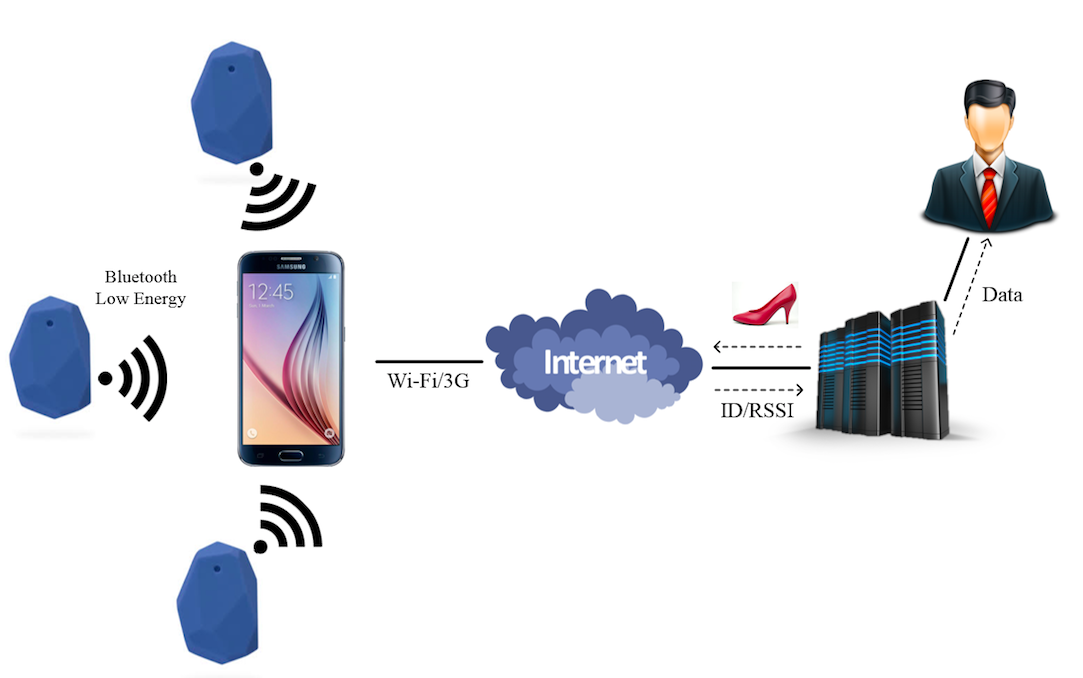
\includegraphics[width=0.9\textwidth]{Figures/architecture.png}
%	\caption[Architecture]{Architecture.}
%	\label{fig:architecture}
%\end{figure}


\section{Beacons}
\label{section:beaconsdesign}

The chosen beacons, due to its battery life and four different values of power intensity, are the ones manufactured by \textit{Shenzen Sky Eletronics Manufactory}.

In order to achieve better results in the calculation of the user's position, beacons must be placed as high as possible since height maximizes coverage of an area and minimizes the attenuation and signal fluctuations that comes from signals being absorbed by people’s bodies. However, if the beacon is too high, geometry starts to work against it, especially if the system is a very localized proximity trigger. Added to this, a higher placement also has the inevitable consequence that it requires ladders or elevated platforms for battery change or a reboot~\citep{Statler}. In Figure~\ref{fig:placement} one can see an example of a local with beacons.

%Escolhemos estes que consequencia têm e apresentar quantidades para area...
When deploying the beacons, there are many parameters to consider, such as: algorithm construction, beacon rate, transmit power, beacon mobility, beacon geometry, beacon density, etc. Performing an exhaustive search of parameter space involves constant beacon redeployment and the result would be highly environment specific. A dense beacon distribution has 1 beacon per 30 $m^{2}$ and a lower density distribution, 1 beacon per 100 $m^{2}$ ~\citep{fingerprintingble}.

\begin{figure}[!htb]
	\centering
	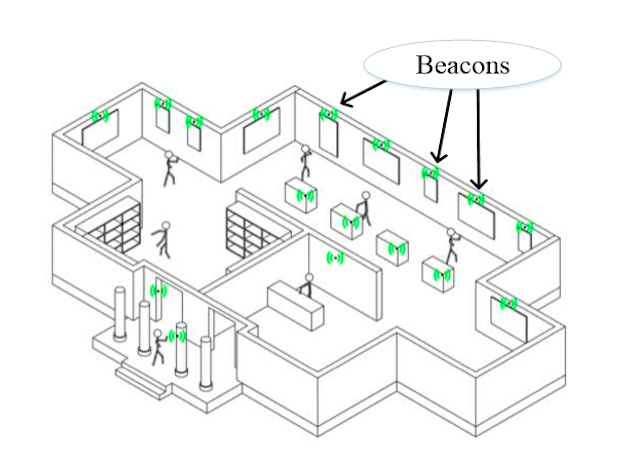
\includegraphics[width=0.9\textwidth]{Figures/placementv2.png}
	\caption[Beacons placement]{Beacons placement.}
	\label{fig:placement}
\end{figure}




\section{Mobile phone Application}
\label{section:app}
The mobile phone application is used by the customer, so it needs to be
user-friendly with an appealing look. When started, the application shows the logotype of the information system and its name. Furthermore, the application shows useful information related to a product or local, links, description or barcodes, Figure~\ref{fig:app_logo} is a template.

\begin{figure}[!htb]
	\centering
	\begin{subfigmatrix}{2}
	\subfigure[Logo]{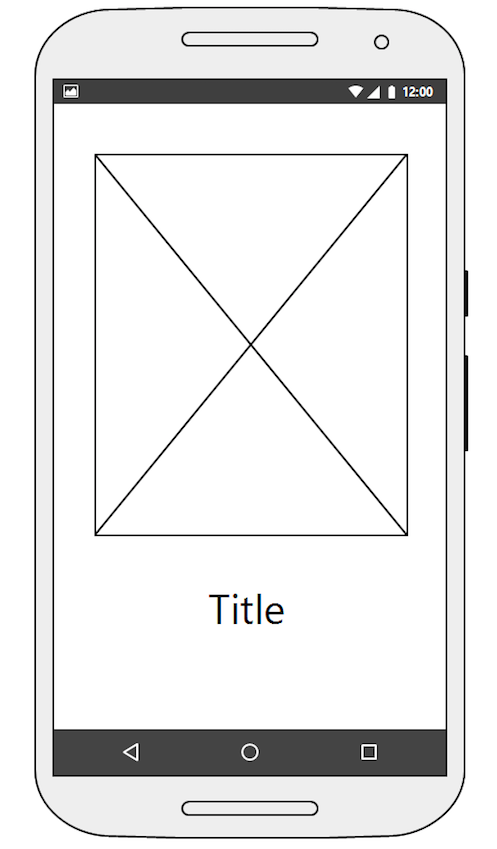
\includegraphics[width=0.35\linewidth]{Figures/logo.png}}
	\subfigure[Product]{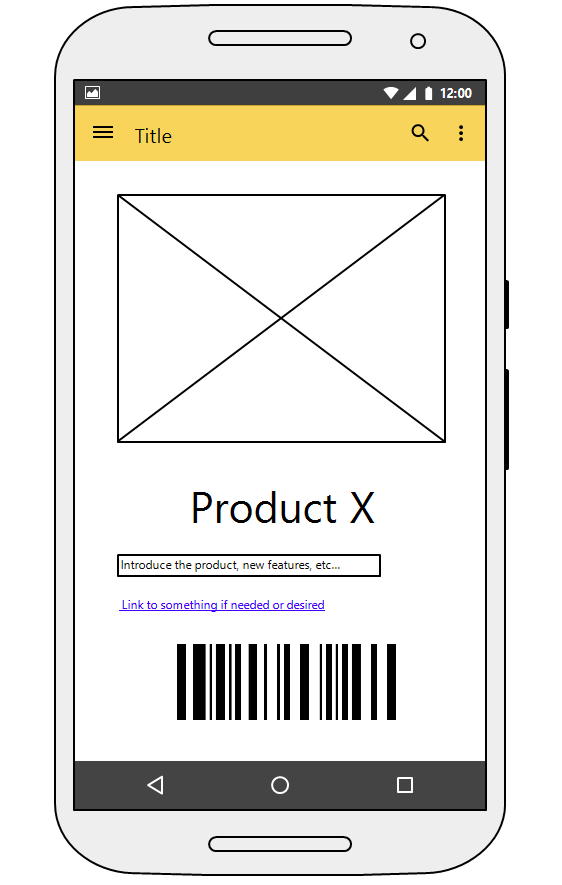
\includegraphics[width=0.38\linewidth]{Figures/product.png}}
	\end{subfigmatrix}
	\caption[Logo and product activities]{Logo and product activities.}
	\label{fig:app_logo}
\end{figure}


Application may have several user profiles, and because of that it can made the sign up and the sign in of the users. These user profiles can be used to save the user's interest or where he has been previously.


\begin{figure}[!htb]
	\centering
	\begin{subfigmatrix}{2}
		\subfigure[Sign up]{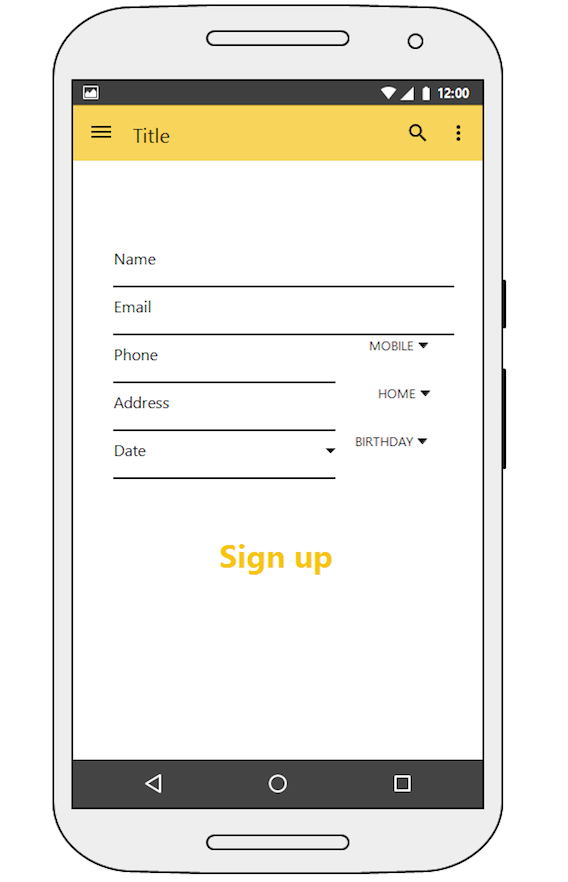
\includegraphics[width=0.39\linewidth]{Figures/signup.png}}
		\subfigure[Sign in]{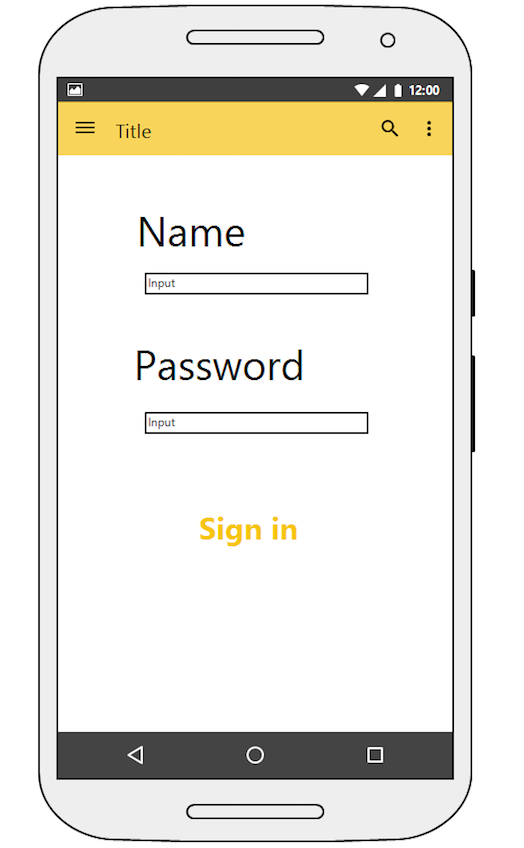
\includegraphics[width=0.37\linewidth]{Figures/signin.png}}
	\end{subfigmatrix}
	\caption[Sign Activities]{Sign Activities.}
	\label{fig:app_sign}
\end{figure}

After, the user is presented with a menu with all the important items or information. Selecting one of them directs the user to its page. In addition to the option to view the list of items, it is also possible to see a map of the location of those items and the user's location, which changes according to his or her position. If the user is close to a specific item, a notification is issued informing the user about the relevant information pertinent to the item . By selecting this notification, it opens an activity to the item information, as shown in Figure~\ref{fig:app_logo}. It should be possible to disable these notifications in the tools button localized in the action bar.


\begin{figure}[!htb]
	\centering
	\begin{subfigmatrix}{2}
		\subfigure[Products list]{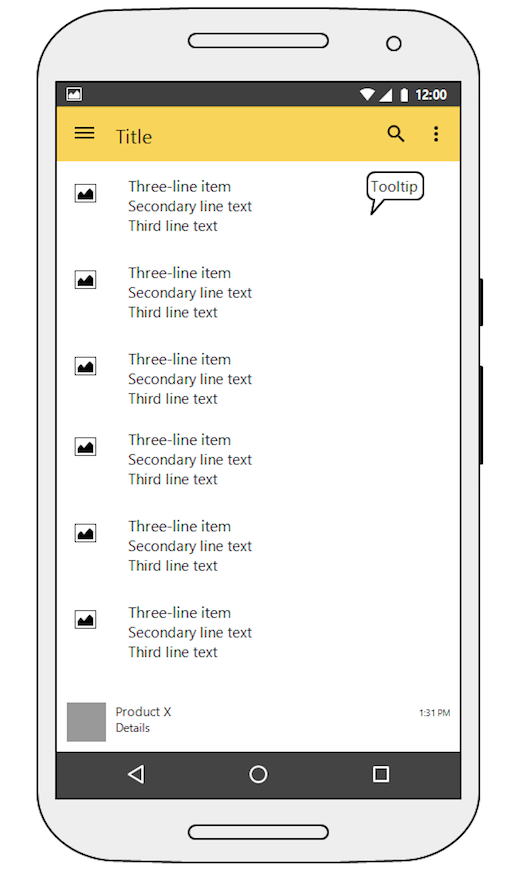
\includegraphics[width=0.35\linewidth]{Figures/list.png}}
		\subfigure[Map]{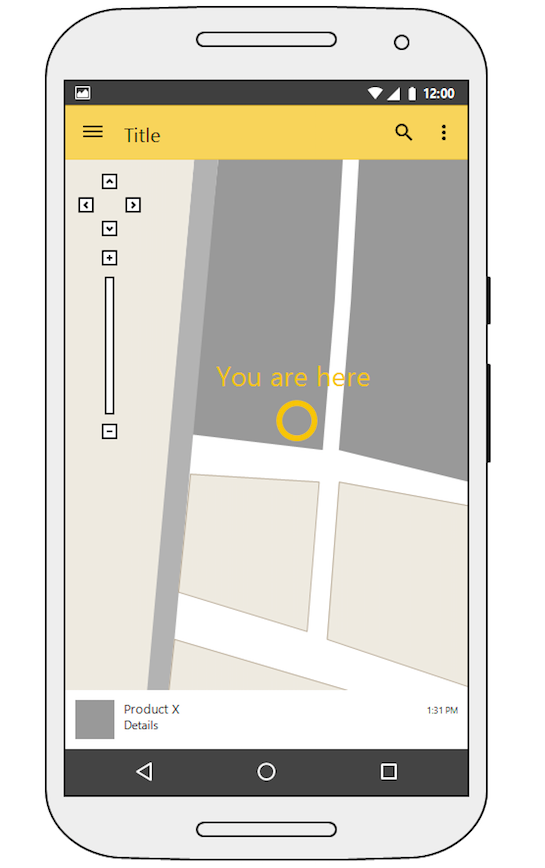
\includegraphics[width=0.38\linewidth]{Figures/map.png}}
	\end{subfigmatrix}
	\caption[Itmes list and Map activities]{Items list and Map activities.}
	\label{fig:app_menu}
\end{figure}

The activities are interconnected and from the first activity it should be possible to move to the register or to the list of items, depending if the user has already signed in. It should be possible to reach the item through the map, notifications or the list.
Figure~\ref{fig:app_story} demonstrates the connection between the activities. The application may send notifications to the user even if it is put in background.
\begin{figure}[!htb]
	\centering
	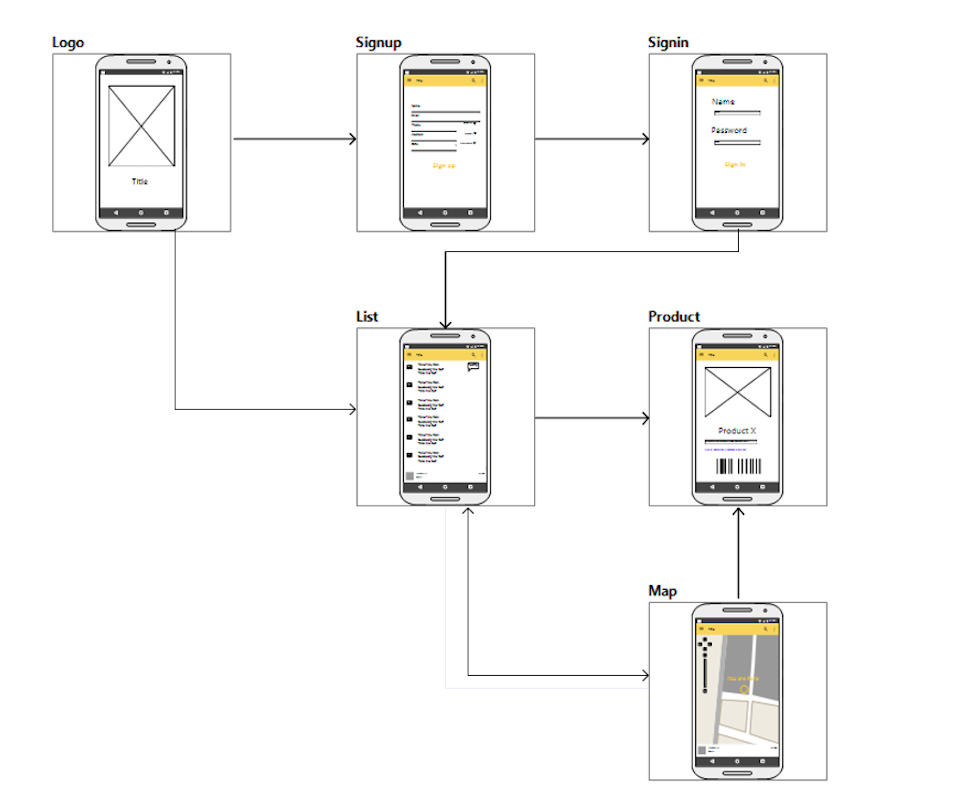
\includegraphics[width=0.85\textwidth]{Figures/story.png}
	\caption[Mobile phone application story]{Mobile phone application story.}
	\label{fig:app_story}
\end{figure}

\section{Back-end}
\label{section:backend}

The back-end has two parts in it: server and database.
The back-end stores all the information related to the user's presence, storing the \gls{rssi} and \gls{uuid} received from the user as well as the accompanying timestamps. It also keeps track of which items the user has selected in the application. This information can be saved in the user profile, if the sign in has been made, or / and saved with the mac address of the user's mobile phone.
It has the map information about the store and where are the items in it.
It has the images of all items and the information that is related to these. 
It responds to the application requests, for updates of the images or description of certain items.
Furthermore, the system owner can access the data collected by the server that is in the database and see this data in an Excel sheet or in a program previously prepared for that task.

Depending on context items can be different things. For instance in a store, items can be products or classes of products, on a museum items can be artworks, on hospitals items can be related to specific areas of expertise. 

\section{Implementation Scenarios}
\label{section:scenarios}
The implementation of the positioning system has two possible scenarios. In the first scenario, we will build a mock-up of context at \gls{ist}, in order to make artificial tests and change the location of the beacons more easily. In the second scenario, we expect to reach an agreement with a commercial enterprise to place the beacons within a location to be defined. FNAC is a possibility since it has a small store at \gls{ist}, but may be open to the implementation of such a setup in a more general setting.

\section{Summary}
\label{section:summary}

The positioning system consists in 3 components: beacons, mobile phone application and back-end. 

The beacons broadcast their \gls{uuid} using the iBeacon protocol. The application listens and collects the \gls{uuid} and their \gls{rssi} and using these the application calculate its position. Then the application sends, from time to time, the user's position to the back-end where it collects the data, recomputes necessary information and sends updates back to the application. The application can have different customer profiles displaying only the information related to the user profile. In the application, the user should have access to a map and a list of all items. The data in the back-end can be accessed by the owner or administrator of the system.

The implementation of the system will have two different scenarios. Initially, the system is deployed at \gls{ist} to make tests. After, the system will be deployed at some store agreed with vendor.